\chapter{Test and Evaluation} \label{sec:tests}

When conceptualizing the tests to be performed, in order to evaluate and validate the solution, the main consideration was to understand how well the solution performed with the constrains made in the hardware and software.

From the moment the final design of the smart shelve was decided, it was evident that two problems could compromise the performance of the solution: the metal structure of shelve and the old, not maintained, Fosstrak open-source software.

In this chapter will be presented a few tests designed to hint how this problems can compromise this solution. The tags were attached to empty sleeves, representing an ideal test environment~\footnote{It was not possible to attain sleeves with aluminum capsules for testing. They would certainty interfere with the following test results, but not accounted in the work of this dissertation.}.

\section{Tag orientation} \label{sec:test1}

Prior to the implementation of the solution, an \ac{rf} analysis of tag orientation in shelve was conducted.
The objective was to evaluate the optimal tag orientation in stored products, and provide notions on system reading performance early in the development.
The tags were tested in tree different orientations, illustrated in figure~\ref{fig:tagorientations}.

\begin{figure}
    \centering
    \caption{Tag orientation tested in this dissertation: horizontal, lateral and vertical, respectively}
    \label{fig:tagorientations}
\end{figure}


This test was only executed on the bottom shelve, since the results could be inferred to the others. The bottom shelve also presented the major challenges and could : it had to operate in the \emph{near-field} and was too close to the antenna, which could cause miss readings in the outer laterals due to the beam width.

The test was conducted by dividing the bottom shelve into $18$ quadrants and measure \ac{rssi} values, referent to a single tag, within those quadrants, with a transmission power of $30$dBm and maximum sensitivity of $-80$dBm. The \ac{rssi} results are a mean value calculated from $1000$ values sampled from each quadrant in a uniform motion, repeated in same manner between quadrants.

The results are shown in figure~\ref{fig:tagorientationsresults} in heatmap plots.
They do not represent the obstructions spread across the shelve. These obstructions prevent tag readings, which were not accounted in this test. Obstructions will be evaluated in the next test.

From the results obtained, there is no clear superior orientation. The circular Keonn Advantenna-p14 in conjunction with the \ac{rf} signal deformations caused by the metal structure, make a good job in providing orientation independence.

\begin{figure}
    \centering
    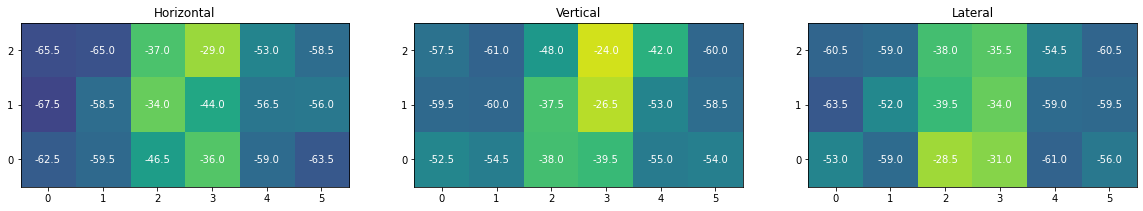
\includegraphics[width=\textwidth]{figs/tests/RSSI_shelve1.png}
    \caption{Tag \ac{rssi} reading results for the different considered orientation. Greater \ac{rssi} values are better.}
    \label{fig:tagorientationsresults}
\end{figure}

A few peculiar observations from the tests are described next:

\begin{itemize}
    \item Horizontal orientated tags have reading problems near the shelf outside metal structure;
    \item Vertical orientated tags, in contrast with horizontal orientated ones, have good reading values near the shelf outside metal structure. They present problems placed on top of the metal bars used to support the shelves.
    \item Lateral orientated tags present difficulty in reader on top of the support metal bars and really close to conners.
\end{itemize}

No major benefits were presented by any orientation.
Theoretically, the lateral tag orientation would present most problems, being parallel to the axis of propagation.
In order to test the system in the most extreme conditions, the lateral orientation was used for sleeves throughout the dissertation and horizontal orientation for product cases for transport.

\section{Shelve \acs{rf} Survey}

The objective of this test is to study and evaluate the certainty and quality of tag readings, by making an \ac{rf} survey of the shelve, with the lateral tag orientation defined previously.
It aims at evaluating the \ac{rf} obstructions present in the solution, which were no considered in the first test.
The results should offer a good representation of the \ac{rf} environment in the shelve and what it could be expected from tag readings in certain locations. 

From the previous test, in section~\ref{sec:test1}, it was observed that the \ac{rssi} does not change when a single tag is placed in one location, allowing the sampling of a single value per location. 

The test consisted, once again, in dividing the shelves into quadrants and measure \ac{rssi} values within those quadrants. This time, each shelve was divided in $140$ quadrants ($20\times7$ grid) to have a better perspective of \ac{rf} obstructions.
The results can be seen in figure~\ref{fig:rfsurvey}.

\begin{figure}
    \centering
    \caption{Heatmap of the \ac{rf} survey measured of each shelf with lateral tag orientation}
    \label{fig:rfsurvey}
\end{figure}

It is possible to observe the obstructions caused from the metal bars used to support the middle of the shelves. The surrounding metal structure does not seem to interfere significantly to the point of blocking readings.

\section{Miss reading stress test}

Test: Accuracy in population of tag readings in blind RF zones.
Objective: Evaluate miss readings in high population tag readings when positioned in poor RF condition locations.
Description: Select poor RF condition locations from Test 1 and for each one at a time, place boxes full of selves in those positions to evaluate for miss readings (result presentation to define).

% ver rfid sourcebook secção rf obstructions

\section{Operational tests}

Test: Platform data validation.
Objective: Validate inventory readings saved in the database.
Description: Make inventory changes and validate through the web interface if the data is in accordance with those changes – namely if tags added or tags retrieved are adequately identified.